\documentclass[11pt,a4paper]{article}
\usepackage{amsmath,amssymb,amsfonts}
\usepackage{graphicx}
\usepackage{hyperref}
\usepackage{geometry}
\usepackage{float}
\usepackage{caption}
\usepackage{subcaption}
\geometry{margin=1in}

\title{\textbf{Relativistic Orbit of the S2 Star in Simpson--Visser Spacetime}}
\author{Preet Dalal}
\date{\today}

\begin{document}
\maketitle

\section*{Overview}

This project investigates the relativistic motion of the S2 star around the compact object at the Galactic Center using the Simpson--Visser (SV) spacetime. The S2 star provides one of the most precise strong-field tests of gravity currently available.   
The goal is to examine whether regular black hole / wormhole geometries can fit the observational data as well as the standard Schwarzschild (SCH) spacetime and to constrain possible deviations from classical General Relativity. 



\section*{Simpson--Visser Spacetime}

The Simpson--Visser metric is a regular spacetime that removes the central curvature singularity through a length scale parameter \(q\). It interpolates between a Schwarzschild black hole and wormhole-like geometries.  For \(q = 0\), the metric reduces exactly to the Schwarzschild spacetime. 

\[
ds^2 = -f(r)\,dt^2 + f(r)^{-1}\,dr^2 + (r^2 + q^2)\,d\Omega^2,
\]
where
\[
f(r) = 1 - \frac{2M}{\sqrt{r^2 + q^2}}, 
\qquad 
d\Omega^2 = d\theta^2 + \sin^2\theta\, d\phi^2
\]
and $M$ being the mass of galactic center. 

The nature of the geometry depends on the value of $q$ relative to $2M$:
\begin{enumerate}
    \item $q = 0$: Schwarzschild black hole with a curvature singularity at $r = 0$;
    \item $0 < q < 2M$: regular black hole with two horizons at $r = \pm \sqrt{(2M)^2 - q^2}$;
    \item $q = 2M$: extremal configuration with a null throat at $r = 0$;
    \item $q > 2M$: two-way traversable wormhole with a timelike throat at $r = 0$. 
\end{enumerate}


\section*{Corner Plots:  SV vs Schwarzschild}

\begin{figure}[H]
\centering
\begin{subfigure}{0.48\textwidth}
  \centering
  \includegraphics[width=\textwidth]{SVBH_corner_plot.png}
  \caption{Simpson--Visser posterior distributions. }
\end{subfigure}
\hfill
\begin{subfigure}{0.48\textwidth}
  \centering
  \includegraphics[width=\textwidth]{SCH_corner_plot.png}
  \caption{Schwarzschild posterior distributions.}
\end{subfigure}
\caption{Corner plots comparing parameter constraints obtained in the Simpson--Visser and Schwarzschild spacetimes.}
\end{figure}



\section*{Relativistic Orbit Fits}

\begin{figure}[H]
\centering
\begin{subfigure}{0.48\textwidth}
  \centering
  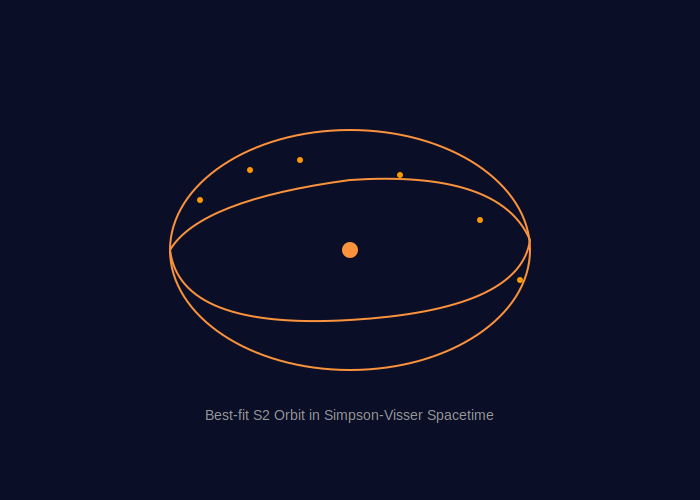
\includegraphics[width=\textwidth]{SVBH_combined. png}
  \caption{Best-fit orbit in Simpson--Visser spacetime. }
\end{subfigure}
\hfill
\begin{subfigure}{0.48\textwidth}
  \centering
  \includegraphics[width=\textwidth]{SCH_combined.png}
  \caption{Best-fit orbit in Schwarzschild spacetime. }
\end{subfigure}
\caption{Sky-projected relativistic orbits of the S2 star.  Points represent observations, and curves show the geodesic solutions.}
\end{figure}


\section*{Constraint on the Simpson--Visser Parameter \(q\)}

From the MCMC analysis, the Simpson--Visser parameter \(q\) (expressed in units of the black hole mass \(M\), with \(M\) measured in million solar masses) is constrained by the S2 star orbital data. 

The upper bounds on the dimensionless ratio \(q/M\) at the \(1\sigma\) and \(2\sigma\) confidence levels are obtained as
\[
\left(\frac{q}{M}\right)_{1\sigma} \leq 2.756 \times 10^{-2},
\]
\[
\left(\frac{q}{M}\right)_{2\sigma} \leq 5.927 \times 10^{-1}.
\]

These bounds place stringent observational limits on the regularization parameter of the Simpson--Visser spacetime.  In particular, they rule out the wormhole branch of the metric as a viable description of the Galactic Center up to the \(2\sigma\) confidence level, thereby favoring black hole–like geometries.

Furthermore, these constraints are significantly tighter than those obtained from black hole shadow observations, where the shadow size remains consistent with all values of \(q\). The S2 star orbit therefore provides a more sensitive probe of the Simpson--Visser parameter and the underlying spacetime geometry. 


\section*{Summary}

\begin{itemize}
  \item A full relativistic orbit-fitting framework is implemented for S2.
  \item Simpson--Visser spacetime provides a statistically competitive fit with Schwarzschild goemetry as 0 $\leq \Delta$AIC $\leq 2$ and 0 $\leq \Delta$BIC $\leq 6$.
  \item The regularization parameter \(q\) is constrained by observational data. 
\end{itemize}

\vspace{0.5cm}
\noindent
\textbf{Status: } Ongoing Research. 

\end{document}